% $Id: Grid_obj.tex,v 1.7 2005/10/21 20:25:18 jwolfe Exp $
%
% Earth System Modeling Framework
% Copyright 2002-2003, University Corporation for Atmospheric Research,
% Massachusetts Institute of Technology, Geophysical Fluid Dynamics
% Laboratory, University of Michigan, National Centers for Environmental
% Prediction, Los Alamos National Laboratory, Argonne National Laboratory,
% NASA Goddard Space Flight Center.
% Licensed under the GPL.

\subsection{Object Model}

The following is a simplified UML diagram showing the structure of the
Grid class.  See Appendix A, {\it A Brief Introduction to UML},
for a translation table that lists the symbols in the diagram and their 
meaning.

\begin{center}
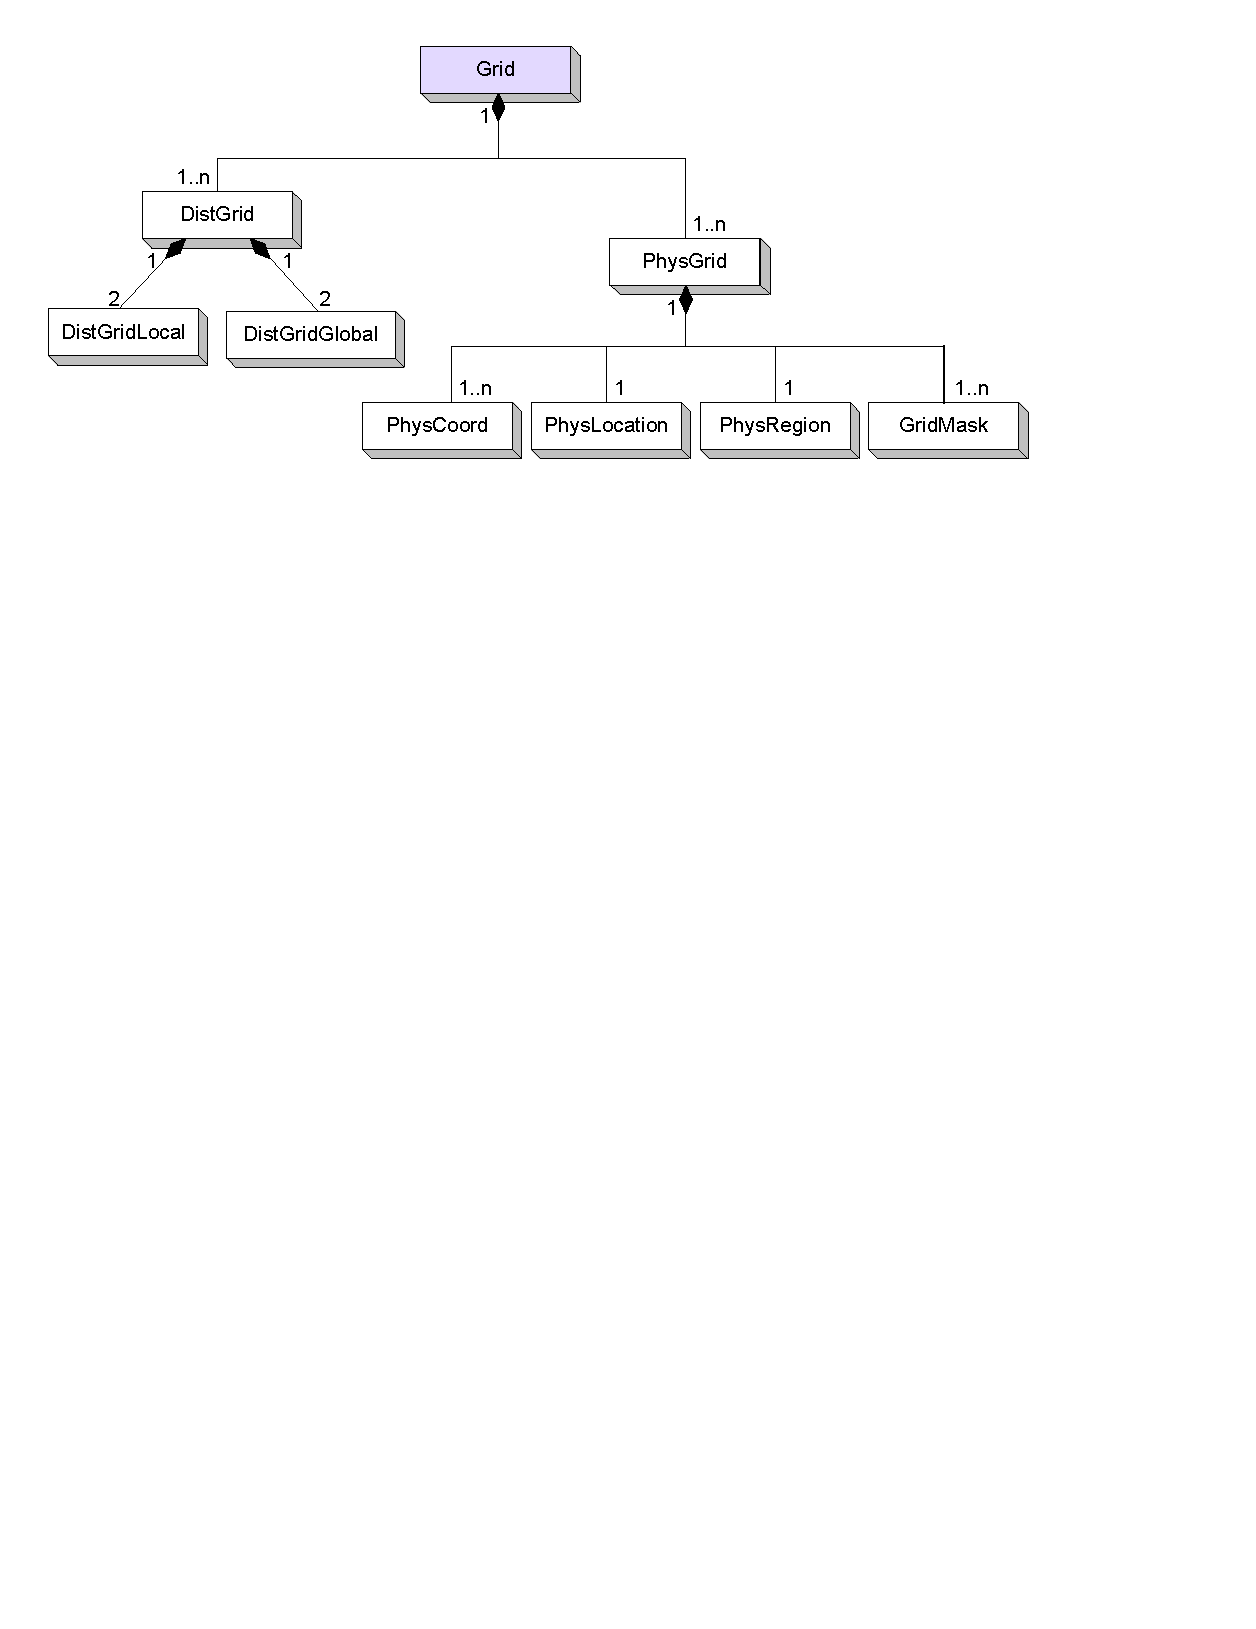
\includegraphics{Grid_obj.eps}   
\end{center}

Each Grid contains at least one Distributed Grid and a related Physical Grid.
The Physical Grid maintains information about the global coordinates.  In
general the coordinates are described implicitly by specifying the grid type
and the corresponding parameters.  However it is possible that the Physical
Grid must be completely enumerated, perhaps in the case of assimilated data
or unstructured data.  The Distributed Grid defines an index space that
corresponds to cells in the Physical Grid and is decomposed among DEs in a
DELayout.  Please see sections \ref{sec:DistGridClasses} and
\ref{sec:PhysGridClasses} for more information about the private
DistGrid and PhysGrid classes.


